% Number 250
% CVPMA Algebra Units
% Tron driving at each other
% JG

% Watermark
\AddToShipoutPicture*{\BackgroundPic}

\addtocounter {ProbNum} {1}

%\begin{floatingfigure}[r]{.3\textwidth}
%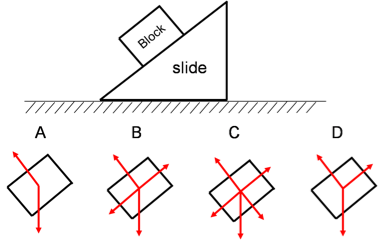
\includegraphics[scale=.4]{/Users/jgates/desktop/latex/pics/incline3.png}
%\end{floatingfigure}
 
{\bf \Large{\arabic{ProbNum}}} Two lightcycles (like from Tron - that movie was awesome, and the remake wasn't bad) charge at each other from an initial distance of 112 meters.  One lightcyle has a constant speed of ${25~\tfrac{m}{s}}$, and the other a constant speed of ${32~\tfrac{m}{s}}$. They drive at each other, barely missing a head-on collision.  

%\begin{center}
%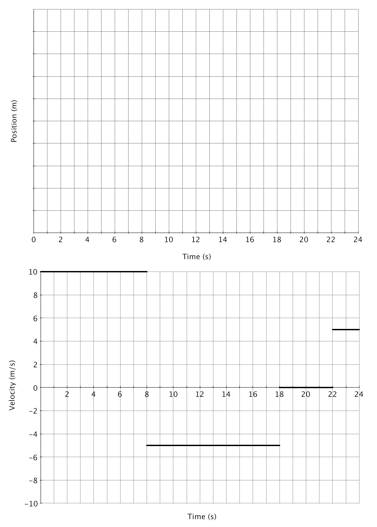
\includegraphics[scale=.77]{/Users/jgates/desktop/latex/pics/vtoxgraph1.png}
%\end{center}

\bigskip
Does CVPM apply? Why or why not?

\vspace{30mm}

How long after they begin driving will they pass each other?
 
\vfill

\newpage